\documentclass[a4paper, 11pt,oneside,openany, danish]{memoir} % Starter dokumentet af klassen memoir


%%%%%%%%%%%%%%%%%%%%%%%
% PREAMBLE %			
%%%%%%%%%%%%%%%%%%%%%%%



% Papirstørrelse og margener
\usepackage[paper=a4paper, hmargin=1.1in, vmargin=1.1in]{geometry}

% Font encoding og sprog
\usepackage[T1]{fontenc}				% Output encoding
\usepackage[utf8]{inputenc}				% Input encoding
\usepackage[danish]{babel}				% Sprog (orddeling)
\renewcommand{\danishhyphenmins}{22} 	% bedre orddeling, minimum to tegn før og efter deling
\usepackage{lmodern}  					% gør underscores pænere
\usepackage{microtype} 					% laver micro ændringer i text for at udgå luft og orddeling


%% Forside text
%\usepackage{soul} % lege lege
%\sodef\an{}{0.2em}{.9em plus.6em}{1em plus.1em minus.1em}
%\newcommand\stext[1]{\an{\scshape#1}}

% Fyldetekst (Lorem ipsum)
\usepackage{blindtext}

% Til kodeeksempler
\usepackage{listings}

\lstdefinestyle{customc}{
	belowcaptionskip=1\baselineskip,
	breaklines=true,
	frame=L,
	xleftmargin=\parindent,
	language=C,
	showstringspaces=false,
	basicstyle=\footnotesize\ttfamily,
	keywordstyle=\bfseries\color{green!40!black},
	commentstyle=\itshape\color{purple!40!black},
	identifierstyle=\color{blue},
	stringstyle=\color{orange},
}

\lstdefinestyle{customasm}{
	belowcaptionskip=1\baselineskip,
	frame=L,
	xleftmargin=\parindent,
	language=[x86masm]Assembler,
	basicstyle=\footnotesize\ttfamily,
	commentstyle=\itshape\color{purple!40!black},
}

\lstset{escapechar=@,style=customc}

% Tabeller
\usepackage{booktabs}
\usepackage{threeparttable}
\usepackage[tableposition=top]{caption}
\usepackage{tabularx}
\usepackage{multirow}					% For at lave pæne tabeller
\usepackage{hhline}						% For at lave endnu pænere tabller
\newcolumntype{C}{>{\let\newline\\\arraybackslash\hspace{0pt}}X}
\usepackage{float}
%matematik
\usepackage{amsmath,amssymb,mathtools,bm}
\newcommand{\tsub}[1]{_{\textup{#1}}}
\def\doubleunderline#1{\underline{\underline{#1}}}
\usepackage[separate-uncertainty = true,multi-part-units=single]{siunitx}
\usepackage{longtable}

% XColor: Farver
\usepackage[svgnames,dvipsnames,x11names]{xcolor}

% Figurer og floats
\usepackage[]{graphicx}
\graphicspath{{figurer/}}
\usepackage{placeins}
\usepackage{float}			% Muliggoer eksakt placering af floats, f.eks. \begin{figure}[H]

%%% Tegning af kasser
%\usepackage{calc,graphicx,color}
%\definecolor{mygreen}{rgb}{0,0.6,0}
%\definecolor{mygray}{rgb}{0.5,0.5,0.5}

% Biblatex til referencer
\usepackage[backend=bibtex]{biblatex}
\addbibresource{bibfil.bib}





% Hyper ref
\usepackage[ unicode=true, colorlinks=false, linktocpage=true, 
pdfborder={0 0 0}, pdfstartpage=1, pdfstartview=FitV, breaklinks=true,
pdfpagemode=UseNone, pageanchor=true, pdfpagemode=UseOutlines,
plainpages=false, bookmarksnumbered, bookmarksopen=true,
bookmarksopenlevel=1, hypertexnames=true, pdfhighlight=/O, urlcolor=Black,
linkcolor=Black, citecolor=Black]{hyperref}

% Clever ref
\usepackage{cleveref}



\settocdepth{subsection}
\setsecnumdepth{subsection}

% Sidetal
% Sidetal
\let\footruleskip\undefined
\usepackage{fancyhdr}
\usepackage{lastpage}
\pagestyle{fancy} 
\fancyhf{} 

\fancyhead[R]{\leftmark}
\fancyfoot[R]{\thepage \hspace{0.008in} af \pageref{LastPage}}

\fancypagestyle{}{
	\renewcommand{\headrulewidth}{0pt}
	\fancyhf{}
	\fancyfoot[R]{\thepage \hspace{0.008in} af \pageref{LastPage}}%
	
}

% Starten på dokumentet
\begin{document}


%%%%%%%%%%%%%%%%%%%%%%%
		       % FORSIDEN %			
%%%%%%%%%%%%%%%%%%%%%%%
% !TEX root = ../prj4projektdokumentation.tex
% SKAL STÅ I TOPPEN AF ALLE FILER FOR AT MASTER-filen KOMPILERES 
\thispagestyle{empty}
{\centering
	{\scshape\LARGE Aarhus Universitet \par}
	\vspace{1cm}
	{\scshape\Large 4. semesterprojekt gruppe 1\par}
	{\scshape\Large Projektdokumentation\par}
	\vspace{1.5cm}
	{\huge\bfseries Spændingsregulator\par}
	\vspace{2cm}
	{\Large
		201509249 - Caroline Møller Sørensen\\
		201611140 - Sophia Amailie Mortensen\\
		201505195 - Dennis Slot Larsen \\
		201505115 - Laurids Givskov Jørgensen\\
		201508333 - Søren Jensen\\
		13114 - Jeppe Hansen\\  }
	\vfill
	Vejleder\par
	Emir Pasic
	
	\vfill
	
	{\large \today\par}
	\par}




\frontmatter
%%%%%%%%%%%%%%%%%%%%%%%

             % RESUME & ABSTRACT %			
             
%%%%%%%%%%%%%%%%%%%%%%%            
\section{Resume}
\section{Abstract}
%%%%%%%%%%%%%%%%%%%%%%%


%%%%%%%%%%%%%%%%%%%%%%%
         % INDHOLDSFORTEGNELSE %			
%%%%%%%%%%%%%%%%%%%%%%%

\tableofcontents

%%%%%%%%%%%%%%%%%%%%%%%
                        % KAPITLER %			
%%%%%%%%%%%%%%%%%%%%%%%                        
\mainmatter
\chapter{Forord}  
% !TEX root =../prj4projektrapport.tex



\textbf{Praktisk information:} I dette projekt deltog seks ingeniørstuderende fra Ingeniørhøjskolen Aarhus Universitet. De studerende er på 4. semester på studieretningen Elektrisk Energiteknologi. Projektgruppens vejleder er Emir Pasic, der løbende har vejledt gruppen. Semesterprojektets afleveringsdato er 29/5-2017 og bedømmelsesdato er 28/6-2017. \\
\textbf{Læsevejledning:} Henvisninger til projektdokumentationen er lavet med fodnoter, der angiver kapitelnummer og navn på det afsnit, der henvises til. Bilagshenvisninger er lavet med mappenavn og bilagsnummer. \\
\textbf{Tak til:} Der skal tilskrives en tak til Michael Rangård, Specialist Planlægning, og Poul Bagger Thomsen, Afdelingsleder Anlæg 20/0,4kV, fra Eniig for hjælp med data og besøg på transformerstation.
                     
\chapter{Indledning}
% !TEX root =../prj4projektrapport.tex

Formålet med dette projekt er at løse følgende problemformulering; \textit{Når belastningerne i et distributionssystem ændres, vil spændingsniveauet variere. Det er vigtigt, at spændingsniveauet holdes stabilt. Hvordan sikres dette?}
Udgangspunktet for problemstillingen er det lovmæssige krav, der siger, at spændingsforsyningen hos danske forbrugere altid skal ligge på 230V $\pm$10$\%$ \cite{Sikkerhedsstyrelsen}. Det ønskes at undersøge udfordringerne ved dette samt at komme med et bud på, hvordan denne problemstilling løses bedst muligt, både som elnettet ser ud i dag, men også i fremtiden. 

For at kunne arbejde med problemformuleringen og undersøge dens aktualitet, valgte projektgruppen at tage kontakt til energiselskabet Eniig. Det viste sig, at der på nuværende tidspunkt ikke foretages regulering på lavspændingsnettet, men i stedet på 60/10 kV transformere. Projektgruppen fandt det derfor interessant at undersøge mulighederne for regulering på lavspændingsnettet og eventuelle fordele og fremtidsaspekter ved dette.

I dette projekt vil fokus derfor være på den del af nettet, der går fra distributionstransformer og ud til forbrugere. For at sikre et stabilt spændingsniveau ønskes det at kunne overvåge tilstanden på distributionslinjen, ikke kun ved transformeren, men også ved hver enkelt forbruger. Det samlede system, der fremstilles i projektet betegnes som Spændingsregulator. Med denne ønskes det at lave et proof of concept i forhold til problemformuleringen. På grund af tilgængelighed af komponenter og udstyr vil prototypen for Spændingsregulator blive skaleret ned. 

For at belyse problemstillingen vil der i dette projekt blive lavet en simulering af en distributionslinje samt belastninger, der skal simulere forbrugere på linjen. Projektet vil desuden bestå af en trintransformer, der giver mulighed for at variere spændingsniveauet til linjen og forbrugerne på sekundærsiden af transformeren.

Til justering af spændingsniveauet, er det nødvendigt at kende til de aktuelle værdier for spændingen både centralt ved trintransformeren og decentralt ved forbrugerne. Af denne grund implementeres enheder til måling af spændingen. Det ønskes desuden at kende til systemets power factor, og derfor skal strømmen også måles. Et eventuelt indhold af harmoniske kan føre til unødig belastning og opvarmning af transformere, og det er derfor fornuftigt at kende til indholdet af harmoniske, og denne parameter skal også måles.
For at kunne holde et ønsket spændingsniveau vil der i projektet implementeres en enhed til regulering af trin på transformeren.

\begin{figure}[H]
	\centering
	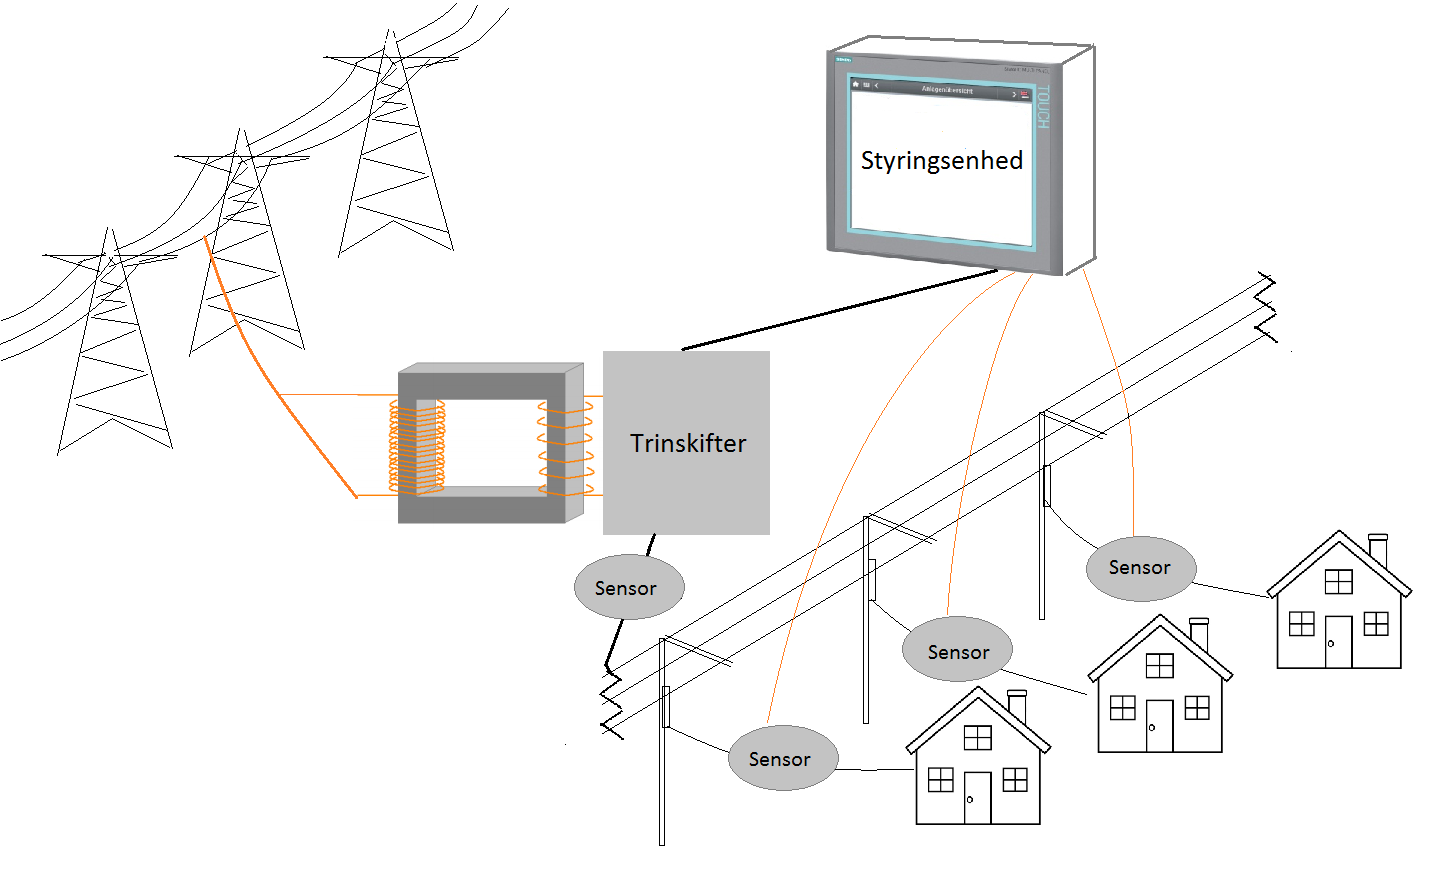
\includegraphics[width=1\textwidth]{figure/RigtBillede}
	\caption{Visuel fremstilling af Spændingsregulator}
	\label{fig:Rigtbillede}
\end{figure}

På figur \ref{fig:Rigtbillede} ses en illustration, der giver oveblik over Spændingsregulatoren. Billedet viser trintransformeren, der forsyner distributionslinjen, sensorer, der måler aktuelle værdier på linjen og en styringsenhed, der regulerer trintransformeren på baggrund af disse værdier. 
\chapter{Kravspecifikation}
% !TEX root = ../prj4projektrapport.tex
% SKAL STÅ I TOPPEN AF ALLE FILER FOR AT MASTER-filen KOMPILERES 

Dette kapitel indeholder en overordnet beskrivelse af systemet, samt en gennemgang af de funktionelle og ikke funktionelle krav der stilles til systemet. 

\section{Systembeskrivelse}
Spændingsregulatoren skal være i stand til at analysere forholdene på distributionslinjen. Derfor udvikles en måleenhed, som kan placeres decentralt, ved hver forbruger, og centralt ved spændingsregulatoren. Måleenhederne skal sende værdier for spænding, strøm, powerfactor og indhold af harmoniske til et system, som regulerer spændingen på baggrund af disse målinger. 

Spændingsreguleringen laves med en trintransformer, hvor der med en styringsenhed kan skiftes mellem trinene. Styringsenheden kan automatisk regulere spændingen jf. data fra måleenhederne, eller den kan styres manuelt på en grafisk brugergrænseflade. 

Systemet der er udviklet i dette projekt er proof of concept, så spændingsniveauet er skalleret ned.  Der er designet et simuleringskredsløb i form af en distributionslinje og en række forbrugere, for at vise funktionaliteten af Spændingsregulatoren. Forbrugerene  kan kobles til/fra nettet, for at generere et spændingsfald der giver anledning til en regulering af trintransformeren. 


% !TEX root = ../../prj4projektdokumentation.tex
% SKAL STÅ I TOPPEN AF ALLE FILER FOR AT MASTER-filen KOMPILERES 

\section{Funktionelle krav}
I dette afsnit beskrives de funktionelle krav for systemet. De dele, hvor en bruger interager med systemet er beskrevet med usecase diagrammer. Den automatiske del er beskrevet og vist vha. et STM diagram.

\subsection{Beskrivelse af automatisk mode}
\label{Afsnit: Automatisk mode}

Når spændingsregulatoren er i automatisk mode, kontrolleres spænding ved forbrugerne. Hvis den spænding er for høj eller lav iht. de 4V skiftes der et trin op eller et trin ned.  
\begin{figure}[htbp] % (alternativt [H])
	\centering
	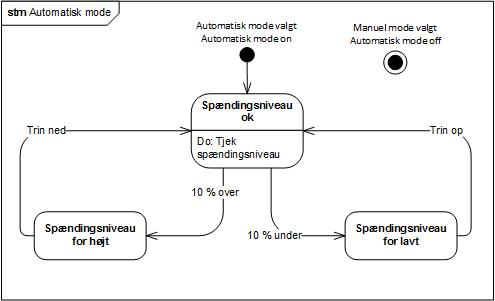
\includegraphics[width=0.8\textwidth]{Figure/STM}
	\caption{Beskrivelse af automatisk mode}
	\label{fig:automode}
\end{figure}

\subsection{Usecase Diagram}

\begin{figure}[H] % (alternativt [H])
	\centering
	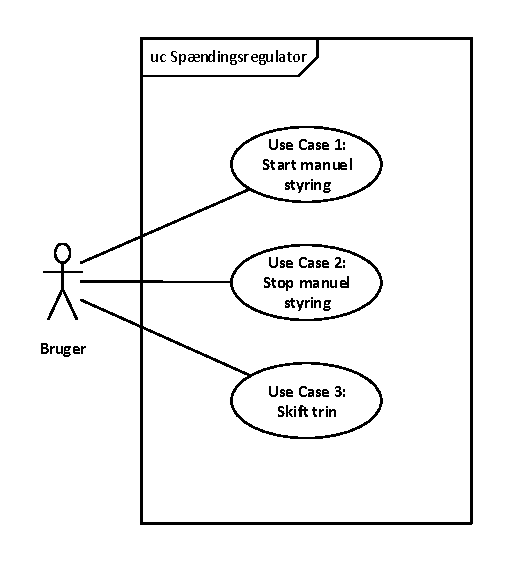
\includegraphics[width=0.5\textwidth]{Figure/UsecaseDiagram}
	\caption{Usecase Diagram}
	\label{fig:UsecaseDiagram}
\end{figure}
Systemet indholder tre usecases, der alle er initieret af brugeren. Den automatiske del af systemet er beskrevet i afsnit \ref{Afsnit: Automatisk mode}.

\subsection{Aktør Beskrivelse}
\textbf{Brugeren} er den primær aktør. En sikkerhedsgodkendt operatør der kan betjene systemet.

\subsection{Usecase 1 - Start manuel styring}
\begin{table}[H]
	\centering
	
	\begin{threeparttable}
		\begin{tabularx}{\linewidth}{ l X }
			\toprule
			\bfseries{Navn:}				& UC1 - Start manuel styring  \\
			\midrule
			\bfseries{Mål:} 				& At sætte systemet i manuel mode \\
			\midrule
			\bfseries{Initiering:} 			& Initieres af brugeren. \\
			\midrule
			\bfseries{Aktører:} 			& Brugeren (Primær) \\
			\midrule
			\bfseries{Samtidige forekomster:} & 1 \\
			\midrule
			\bfseries{Forudsætninger:} 		& At systemet er funktionelt og i automatisk mode\\
			\midrule
			\bfseries{Resultat:} 			& Systemet er i manuel mode \\
			\midrule
			\bfseries{Hovedscenariet:} 	& \\
			
			
			1 	& Brugeren trykker Manuel styring på skærmen.\\
			2	& Systemet skifter til Manuel mode. \\
			3 	& Systemet aktivere manuel skærm. 	\\
			
			\bottomrule
			
		\end{tabularx}
	\end{threeparttable}
	\caption{Fully dressed use case for UC1 - Start manuel styring}
	\label{table:UC1}
\end{table}

\subsection{Usecase 2 - Stop manuel styring}

\begin{table}[H]
	\centering
	
	\begin{threeparttable}
		\begin{tabularx}{\linewidth}{ l X }
			\toprule
			\bfseries{Navn:}				& UC2 - Stop manuel styring  \\
			\midrule
			\bfseries{Mål:} 				& At sætte systemet i automatisk mode \\
			\midrule
			\bfseries{Initiering:} 			& Initieres af brugeren. \\
			\midrule
			\bfseries{Aktører:} 			& Brugeren (Primær) \\
			\midrule
			\bfseries{Samtidige forekomster:} & 1 \\
			\midrule
			\bfseries{Forudsætninger:} 		& At systemet er funktionelt og i manuel mode\\
			\midrule
			\bfseries{Resultat:} 			& Systemet er i automatisk mode \\
			\midrule
			\bfseries{Hovedscenariet:} 	& \\
			
			
			1 	& Brugeren trykker Automatisk styring på skærmen.\\
			2 	& Systemet skifter til Automatisk mode.\\
			3 	& Systemet aktivere automatisk skærm. 	\\		
				
			
			\bottomrule
			
		\end{tabularx}
	\end{threeparttable}
	\caption{Fully dressed use case for UC2 - Stop manuel styring}
	\label{table:UC2}
\end{table}

\subsection{Usecase 3a - Skift trin}

\begin{table}[H]
	\centering
	
	\begin{threeparttable}
		\begin{tabularx}{\linewidth}{ l X }
			\toprule
			\bfseries{Navn:}				& UC3a - Skift trin op  \\
			\midrule
			\bfseries{Mål:} 				& At skifte et trin op på transformeren \\
			\midrule
			\bfseries{Initiering:} 			& Initieres af brugeren. \\
			\midrule
			\bfseries{Aktører:} 			& Brugeren (Primær) \\
			\midrule
			\bfseries{Samtidige forekomster:} & 1 \\
			\midrule
			\bfseries{Forudsætninger:} 		& At systemet er funktionelt og i manuel mode\\
			\midrule
			\bfseries{Resultat:} 			& Transformerens trin er skiftet et trin op \\
			\midrule
			\bfseries{Hovedscenariet:} 	& \\
			
			
			1 	& Brugeren vælger Trin Op på skærmen.\\
			2 	& Systemet skifter et trin op på transformeren.\\
			3 	& Aktuelt trin vises på skærmen.\\
			4 	& Måleværdier opdateres på skærmen.\\		
			
			\bottomrule
			
		\end{tabularx}
	\end{threeparttable}
	\caption{Fully dressed use case for UC3 - Skift trin}
	\label{table:UC3}
\end{table}

\subsection{Usecase 3b - Skift trin}

\begin{table}[H]
	\centering
	
	\begin{threeparttable}
		\begin{tabularx}{\linewidth}{ l X }
			\toprule
			\bfseries{Navn:}				& UC3b - Skift trin ned  \\
			\midrule
			\bfseries{Mål:} 				& At skifte et trin ned på transformeren \\
			\midrule
			\bfseries{Initiering:} 			& Initieres af brugeren. \\
			\midrule
			\bfseries{Aktører:} 			& Brugeren (Primær) \\
			\midrule
			\bfseries{Samtidige forekomster:} & 1 \\
			\midrule
			\bfseries{Forudsætninger:} 		& At systemet er funktionelt og i manuel mode\\
			\midrule
			\bfseries{Resultat:} 			& Transformerens trin er skiftet et trin ned \\
			\midrule
			\bfseries{Hovedscenariet:} 	& \\
			
			
			1 	& Brugeren vælger Trin Ned på skærmen.\\
			2 	& Systemet skifter et trin ned på transformeren.\\
			3 	& Aktuelt trin vises på skærmen.\\
			4 	& Måleværdier opdateres på skærmen.\\			
			
			\bottomrule
			
		\end{tabularx}
	\end{threeparttable}
	\caption{Fully dressed use case for UC3 - Skift trin}
	\label{table:UC3}
\end{table}



% !TEX root = ../prj4projektrapport.tex
% SKAL STÅ I TOPPEN AF ALLE FILER FOR AT MASTER-filen KOMPILERES 

\section{Ikke Funktionelle Krav}

% !TEX root = ../prj4projektrapport.tex
% SKAL STÅ I TOPPEN AF ALLE FILER FOR AT MASTER-filen KOMPILERES 


\section{Afgrænsning}
Afgrænsning af projektet er lavet som MoSCoW. Der beskrives hvad, der skal med i projektet, for at det fungere og hvad der ikke er så vigtigt. Der er i projektet ikke taget højde for optimering, men kun at der skal være et færdigt funktionelt produkt.
\subsubsection{MoSCoW}

\begin{itemize}
	\item{Systemet \textbf{skal} bestå af en trinskifter 24/0-8V}
	\item{Systemet \textbf{skal} måle spænding, strøm, power factor og harmoniske centralt og decentralt}
	\item{Systemet \textbf{skal} vise data på en skærm}
	\item{Systemet \textbf{skal} simulere en distributionslinje og flere forbrugere}
	\item{Systemet \textbf{skal} kunne reguleres manuelt}
	\item{Systemet \textbf{burde} kunne reguleres automatisk}
	\item{Systemet \textbf{kunne} have en log}
	\item{Distributionslinjen \textbf{kunne} indeholde en decentral producent}
	\item{Systemet \textbf{vil ikke} fjerne harmoniske} 
\end{itemize}	
\chapter{Arkitektur}
% !TEX root =../prj4projektrapport.tex

Formålet med dette projekt er at løse følgende problemformulering; \textit{Når belastningerne i et distributionssystem ændres, vil spændingsniveauet variere. Det er vigtigt, at spændingsniveauet holdes stabilt. Hvordan sikres dette?}
Udgangspunktet for problemstillingen er det lovmæssige krav, der siger, at spændingsforsyningen hos danske forbrugere altid skal ligge på 230V $\pm$10$\%$ \cite{Sikkerhedsstyrelsen}. Det ønskes at undersøge udfordringerne ved dette samt at komme med et bud på, hvordan denne problemstilling løses bedst muligt, både som elnettet ser ud i dag, men også i fremtiden. 

For at kunne arbejde med problemformuleringen og undersøge dens aktualitet, valgte projektgruppen at tage kontakt til energiselskabet Eniig. Det viste sig, at der på nuværende tidspunkt ikke foretages regulering på lavspændingsnettet, men i stedet på 60/10 kV transformere. Projektgruppen fandt det derfor interessant at undersøge mulighederne for regulering på lavspændingsnettet og eventuelle fordele og fremtidsaspekter ved dette.

I dette projekt vil fokus derfor være på den del af nettet, der går fra distributionstransformer og ud til forbrugere. For at sikre et stabilt spændingsniveau ønskes det at kunne overvåge tilstanden på distributionslinjen, ikke kun ved transformeren, men også ved hver enkelt forbruger. Det samlede system, der fremstilles i projektet betegnes som Spændingsregulator. Med denne ønskes det at lave et proof of concept i forhold til problemformuleringen. På grund af tilgængelighed af komponenter og udstyr vil prototypen for Spændingsregulator blive skaleret ned. 

For at belyse problemstillingen vil der i dette projekt blive lavet en simulering af en distributionslinje samt belastninger, der skal simulere forbrugere på linjen. Projektet vil desuden bestå af en trintransformer, der giver mulighed for at variere spændingsniveauet til linjen og forbrugerne på sekundærsiden af transformeren.

Til justering af spændingsniveauet, er det nødvendigt at kende til de aktuelle værdier for spændingen både centralt ved trintransformeren og decentralt ved forbrugerne. Af denne grund implementeres enheder til måling af spændingen. Det ønskes desuden at kende til systemets power factor, og derfor skal strømmen også måles. Et eventuelt indhold af harmoniske kan føre til unødig belastning og opvarmning af transformere, og det er derfor fornuftigt at kende til indholdet af harmoniske, og denne parameter skal også måles.
For at kunne holde et ønsket spændingsniveau vil der i projektet implementeres en enhed til regulering af trin på transformeren.

\begin{figure}[H]
	\centering
	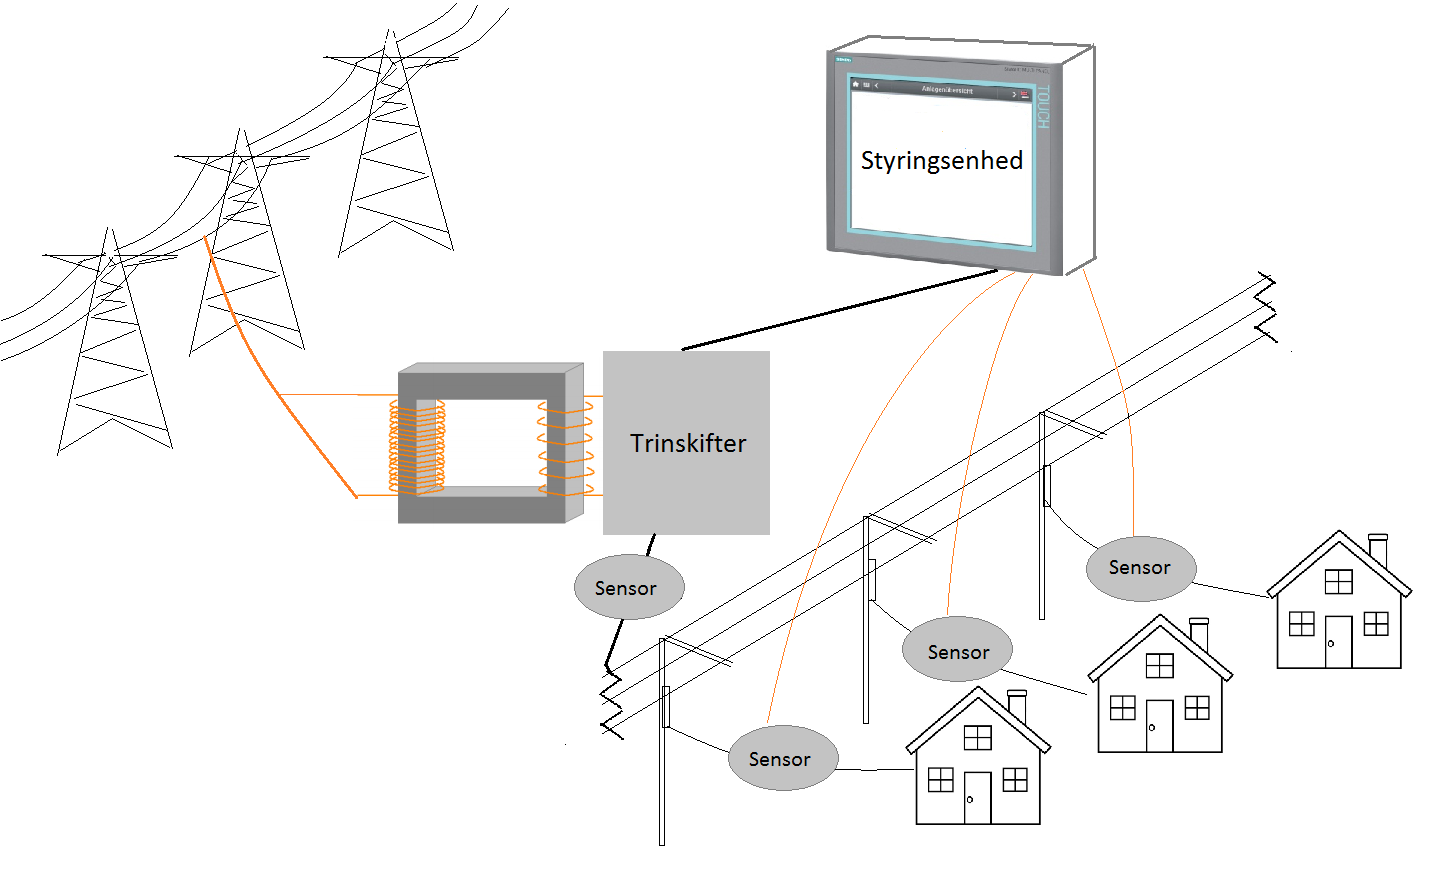
\includegraphics[width=1\textwidth]{figure/RigtBillede}
	\caption{Visuel fremstilling af Spændingsregulator}
	\label{fig:Rigtbillede}
\end{figure}

På figur \ref{fig:Rigtbillede} ses en illustration, der giver oveblik over Spændingsregulatoren. Billedet viser trintransformeren, der forsyner distributionslinjen, sensorer, der måler aktuelle værdier på linjen og en styringsenhed, der regulerer trintransformeren på baggrund af disse værdier. 
% !TEX root = ../../prj4projektdokumentation.tex
% SKAL STÅ I TOPPEN AF ALLE FILER FOR AT MASTER-filen KOMPILERES 

\section{Blok definitionsdiagram}
Et BDD for spændingsregulator ses på figur \ref{fig:BDDSpaendingsregulator}. På diagrammet ses de overordnet blokke spædingsregulator består af. En beskrivelse af hver blok kan læses under figur \ref{fig:BDDSpaendingsregulator}.

\begin{figure}[htbp] % (alternativt [H])
	\centering
	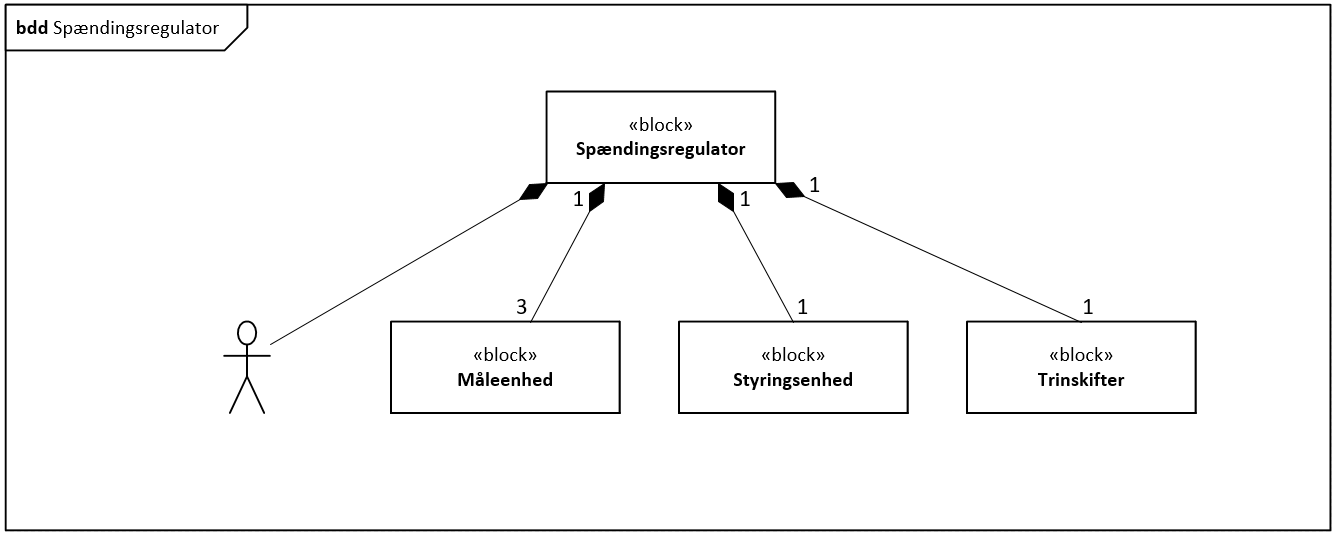
\includegraphics[width=0.9\textwidth]{Figure/BDDSpaendingsregulator}
	\caption{BDD Spændingsregulator}
	\label{fig:BDDSpaendingsregulator}
\end{figure}

\textbf{Måleenhed} står for at måle spænding, strøm og faseforskydningen herimellem. Ligeledes skal denne kunne måle indeholdet af harmoniske frekvenser. Den består af hardware til måling af de nævnte parametre og en PSoC 5. På enheden ligger også en del af behandlingen af rådataet, så dette kan formidles til styringsenheden.

\textbf{Styringsenhed} har til opgave at styre trinskifteren ud fra de data den får fra målenehderne. Den består af en PLC, tl styringen og et HMI, der skal give en bruger overblik over status for distributionslinjen.

\textbf{Trinskifter} er en enhed der kan skifte trin på transformeren ud fra et signal fra styringsenheden. Den består altå af en kontakt for hvert trin, der kan kontrolleres af styringsenheden.
% !TEX root = ../../prj4projektdokumentation.tex
% SKAL STÅ I TOPPEN AF ALLE FILER FOR AT MASTER-filen KOMPILERES 

\section{Intern blok diagram}
På figur \ref{fig:IBDSp} og figur \ref{fig:IBDSt} ses IBD for henholdsvis Spændingsregulator og Styringsenhed. På diagrammerne ses de interne forbindelser i systemet. Under figurne er tilhørende signalbeskrivelser, se tabel \ref{tab:SignalbeskrivelseSp} og tabel \ref{tab:SignalbeskrivelseSt}, der uddyber diagrammerne nærmere.

\begin{figure}[htbp] % (alternativt [H])
	\centering
	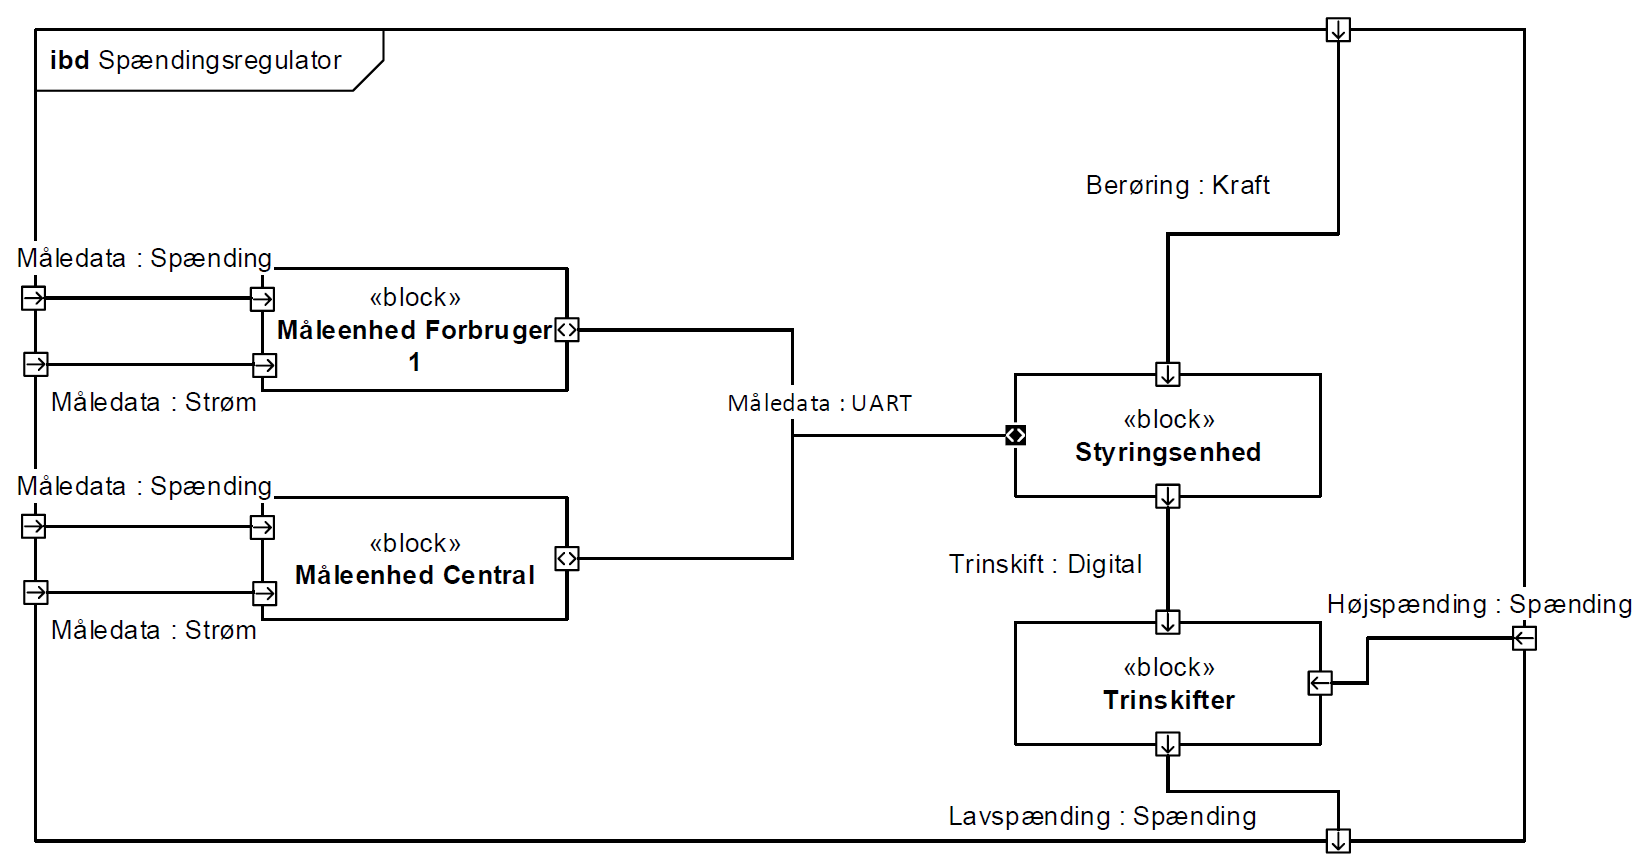
\includegraphics[width=0.8\textwidth]{Figure/IBDSpaendingsregulator1}
	\caption{IBD for Spændingsregulator}
	\label{fig:IBDSp}
\end{figure}

\begin{table}[H]
	\centering
	\begin{tabular}{|l|l|l|l|p{4cm}|}
		\hline
		\textbf{Blok} & \textbf{Navn} & \textbf{Type} & \textbf{Signal} & 
		\textbf{Beskrivelse} \\\hline
		
		\multirow{3}{*}{Måleenhed} 
		& Måledata & Spænding & In & Måledata er spændingsniveauet på distributionslinjen. \\\hhline{~----} 
		& Måledata & Strøm & In & Måledata er strømniveauet på distributionslinjen. \\\hhline{~----} 
		& Måledata & UART & InOut & UART forbindelse til Styringsenhed \\\hline
		
		\multirow{3}{*}{Styringsenhed} 
		& Måledata & UART & Inout & UART forbindelse til Måleenhed \\\hhline{~----} 
		& Berøring & Kraft & In & Tryk på Brugergrænseflade \\\hhline{~----} 
		& Trinskift & Digital & Out & Trinskift er en digital kommando til Trinskifter \\\hline
		
		\multirow{3}{*}{Trinskifter} 
		& Trinskift & Digital & In & Trinskift er en digital kommando fra Styringsenhed. \\\hhline{~----} 
		& Højspænding & Spænding & In & Er spændingen på højspændingssiden af tranformeren. \\\hhline{~----} 
		& Lavspænding & Spænding & Out & Er spændingen på lavspændingssiden af transformeren. \\\hline
	\end{tabular}
	\caption{Signalbeskrivelse for Spændingsregulator}
	\label{tab:SignalbeskrivelseSp}
	
\end{table}


\begin{figure}[htbp] % (alternativt [H])
	\centering
	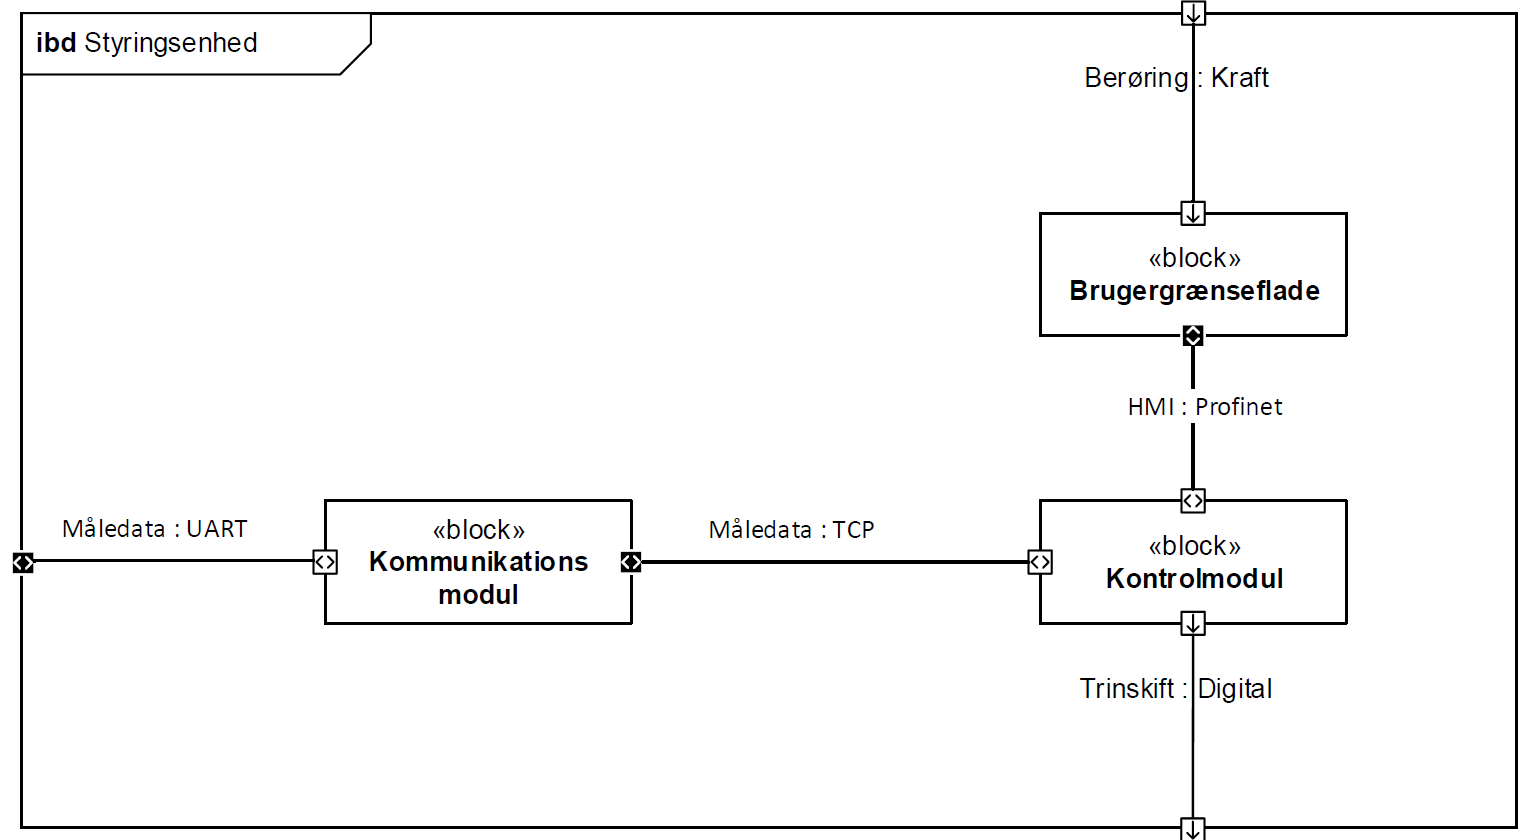
\includegraphics[width=0.8\textwidth]{Figure/IBDStyringsenhed1}
	\caption{IBD for Styringsenhed}
	\label{fig:IBDSt}
\end{figure}

\begin{table}[H]
	\centering
	\begin{tabular}{|l|l|l|l|p{4cm}|}
		\hline
		\textbf{Blok} & \textbf{Navn} & \textbf{Type} & \textbf{Signal} & 
		\textbf{Beskrivelse} \\\hline
		
		\multirow{2}{*}{Brugergrænseflade} 
		& Berøring & Kraft & In & Tryk på Brugergrænseflade \\\hhline{~----} 
		& HMI & Profinet & InOut & Forbindelse til Kontrolmodul \\\hline
		
		\multirow{3}{*}{Kontrolmodul} 
		& HMI & Profinet & InOut & Forbindelse til Brugergrænseflade \\\hhline{~----} 
		& Trinskift & Digital & Out & Trinskift er en digital kommando til Trinskifter \\\hhline{~----} 
		& Måledata & TCP & InOut & TCP forbindelse til Kommunikationsmodul \\\hline
		
		\multirow{2}{*}{Kommunikationsmodul} 
		& Måledata & TCP & InOut & TCP forbindelse til Kontrolmodul \\\hhline{~----} 
		& Måledata & UART & InOut & UART forbindelse til Måleenhed \\\hline
	\end{tabular}
	\caption{Signalbeskrivelse for Styringsenhed}
	\label{tab:SignalbeskrivelseSt}
	
\end{table}


\newpage
% !TEX root = ../../prj4projektrapport.tex
% SKAL STÅ I TOPPEN AF ALLE FILER FOR AT MASTER-filen KOMPILERES 


\section{Allokeringsdiagram}

Herunder ses allokeringsdiagrammet udviklet for systemet. Diagrammet er udviklet for at give et overblik over udviklingen af software og kommunikation i projektet. Et allokeringsdiagram giver et indblik i hvor forskellige dele af projektets funktionalitet skal programmeres, samt hvordan de enkelte enheder kommunikerer sammen. For yderlig beskrivelse af diagrammet se dokumentation\footnote{Projektdokumentation, 5.3, Allokeringsdiagram}.


\begin{figure}[htbp] % (alternativt [H])
	\centering
	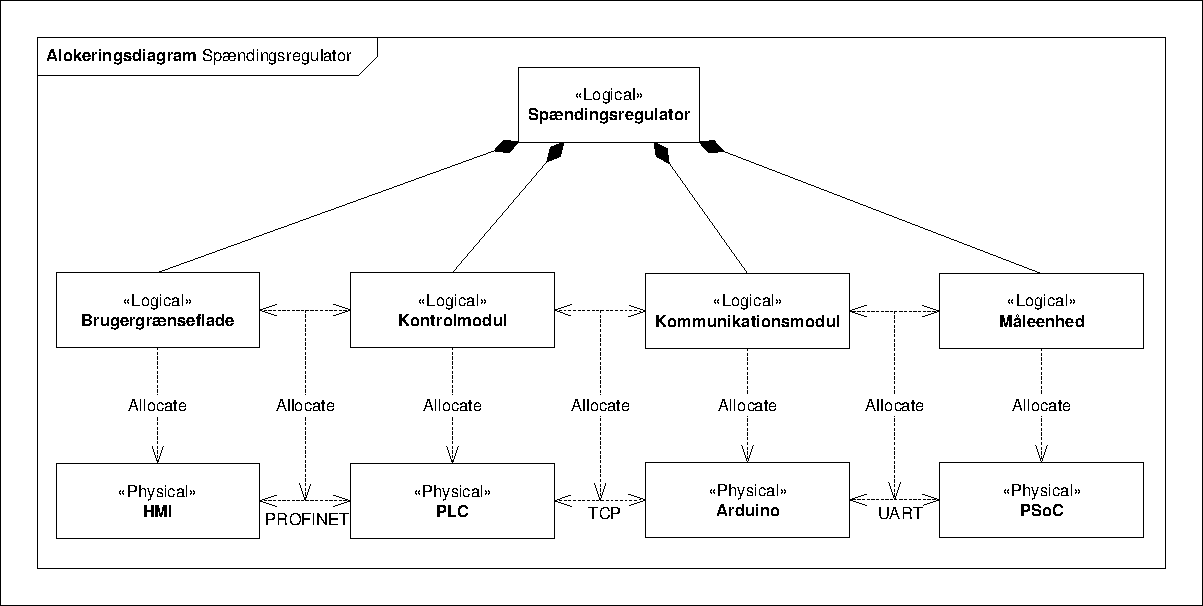
\includegraphics[width=0.8\textwidth]{figure/Allokering.pdf}
	\caption{Allokeringsdiagram for Spændingsregulator}
	\label{fig:Allokering}
\end{figure}
\chapter{Design af distributionslinje, belastning og trinskifter}
\chapter{Design af Måleenhed}
\chapter{Design af Styringsenhed}
% !TEX root =../prj4projektrapport.tex

Formålet med dette projekt er at løse følgende problemformulering; \textit{Når belastningerne i et distributionssystem ændres, vil spændingsniveauet variere. Det er vigtigt, at spændingsniveauet holdes stabilt. Hvordan sikres dette?}
Udgangspunktet for problemstillingen er det lovmæssige krav, der siger, at spændingsforsyningen hos danske forbrugere altid skal ligge på 230V $\pm$10$\%$ \cite{Sikkerhedsstyrelsen}. Det ønskes at undersøge udfordringerne ved dette samt at komme med et bud på, hvordan denne problemstilling løses bedst muligt, både som elnettet ser ud i dag, men også i fremtiden. 

For at kunne arbejde med problemformuleringen og undersøge dens aktualitet, valgte projektgruppen at tage kontakt til energiselskabet Eniig. Det viste sig, at der på nuværende tidspunkt ikke foretages regulering på lavspændingsnettet, men i stedet på 60/10 kV transformere. Projektgruppen fandt det derfor interessant at undersøge mulighederne for regulering på lavspændingsnettet og eventuelle fordele og fremtidsaspekter ved dette.

I dette projekt vil fokus derfor være på den del af nettet, der går fra distributionstransformer og ud til forbrugere. For at sikre et stabilt spændingsniveau ønskes det at kunne overvåge tilstanden på distributionslinjen, ikke kun ved transformeren, men også ved hver enkelt forbruger. Det samlede system, der fremstilles i projektet betegnes som Spændingsregulator. Med denne ønskes det at lave et proof of concept i forhold til problemformuleringen. På grund af tilgængelighed af komponenter og udstyr vil prototypen for Spændingsregulator blive skaleret ned. 

For at belyse problemstillingen vil der i dette projekt blive lavet en simulering af en distributionslinje samt belastninger, der skal simulere forbrugere på linjen. Projektet vil desuden bestå af en trintransformer, der giver mulighed for at variere spændingsniveauet til linjen og forbrugerne på sekundærsiden af transformeren.

Til justering af spændingsniveauet, er det nødvendigt at kende til de aktuelle værdier for spændingen både centralt ved trintransformeren og decentralt ved forbrugerne. Af denne grund implementeres enheder til måling af spændingen. Det ønskes desuden at kende til systemets power factor, og derfor skal strømmen også måles. Et eventuelt indhold af harmoniske kan føre til unødig belastning og opvarmning af transformere, og det er derfor fornuftigt at kende til indholdet af harmoniske, og denne parameter skal også måles.
For at kunne holde et ønsket spændingsniveau vil der i projektet implementeres en enhed til regulering af trin på transformeren.

\begin{figure}[H]
	\centering
	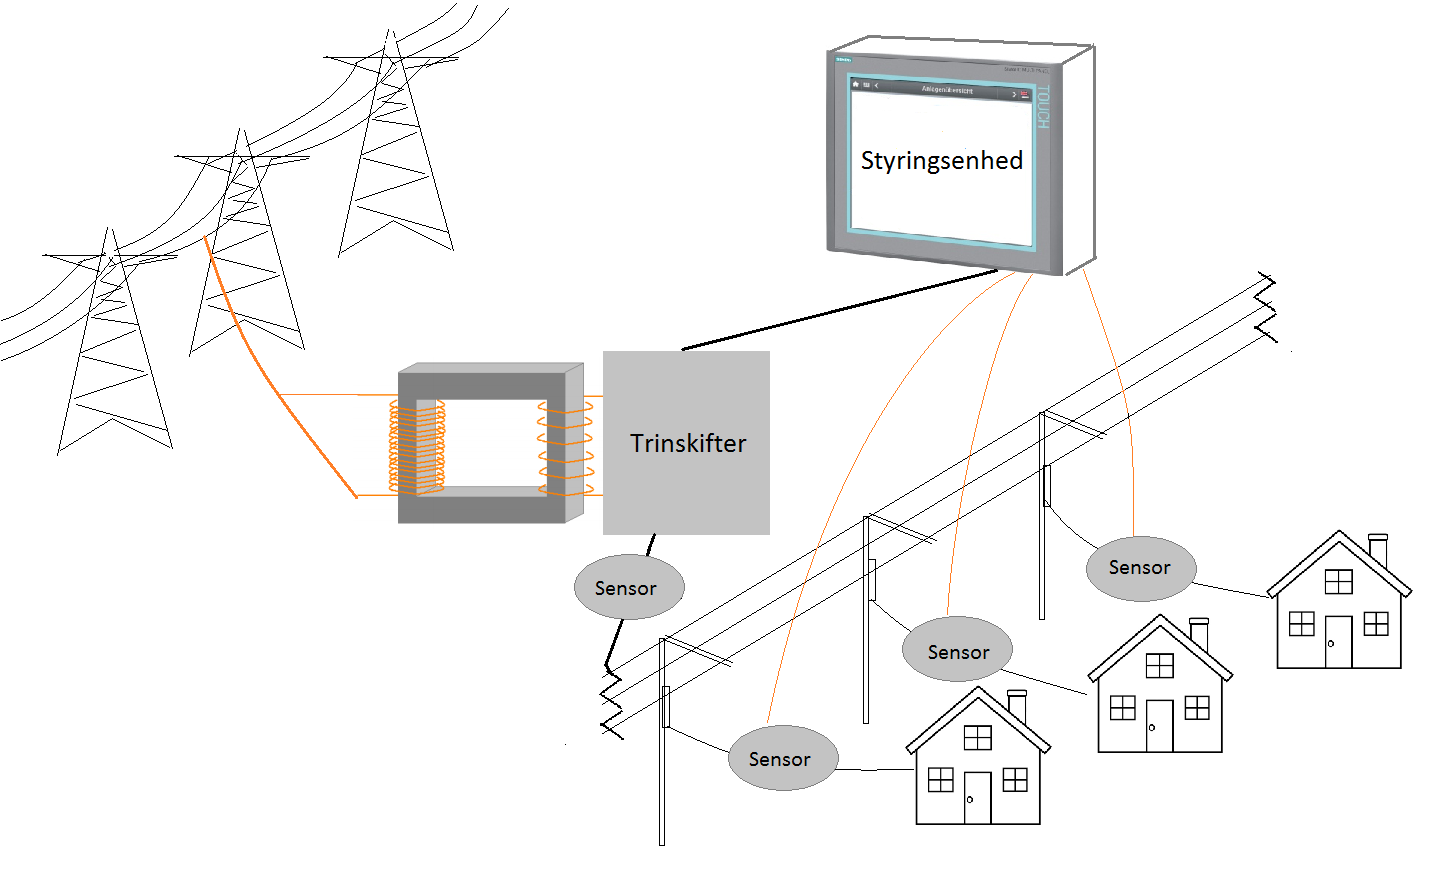
\includegraphics[width=1\textwidth]{figure/RigtBillede}
	\caption{Visuel fremstilling af Spændingsregulator}
	\label{fig:Rigtbillede}
\end{figure}

På figur \ref{fig:Rigtbillede} ses en illustration, der giver oveblik over Spændingsregulatoren. Billedet viser trintransformeren, der forsyner distributionslinjen, sensorer, der måler aktuelle værdier på linjen og en styringsenhed, der regulerer trintransformeren på baggrund af disse værdier. 
% !TEX root = ../../prj4projektrapport.tex
% SKAL STÅ I TOPPEN AF ALLE FILER FOR AT MASTER-filen KOMPILERES 

\section{Foranalyse for Styringsenhed}

\subsection{Kontrolmodul og Brugergrænseflade}
Det er en oplagt mulighed at anvende en PLC og et HMI, som Kontrolmodul og Brugergrænseflade i projektet. Dette skyldes at der, som krav til projektet skulle anvendes relevante faglige elementer fra semestrets kurser. Faget Instrumentering og Automatisering(IOA) omhandler netop brugen af PLC og HMI i industrien. Hermed kommer to gode argumenter for PLC og HMI; relevant faglige viden anvendes og i den virkelige verden ville det være oplagt at bruge lignende enheder til et projekt som dette.


PLC'en kan programmeres i flere forskellig sprog. Ladder er dog blevet valgt, fordi det er det mest anvendte i IOA. Desuden er det et krav til projektet at en bruger skal kunne interagere med systemet, hvilket opnåes gennem HMI'et.


Kravet om pålidelig transmission af data mellem udvalgte enheder understøtter også valget af en PLC, da denne indeholder mulighed for LAN kommunikation gennem en RJ-45 port.

\subsection{Kommunikationsmodul}
Det blev hurtigt i projektfasen valgt at der skulle udvikles kommunikation over en LAN forbindelse, da det i projektet var et krav at der skal være pålidelig transmission af data mellem udvalgte enheder. Der blev undersøgt hvilke muligheder der var for at gøre kommunikation over en LAN forbindelse med en microcontroller muligt, da vi allerede havde haft PSoC og Arduino programmering blev der i Embedded Stock bestilt et ethernet shield til hver af disse. Men da Måleenheden bliver implementeret på en PSoC blev det besluttet at prøve at implementere LAN kommunikationen på samme PSoC, som en af Måleenhederne. 


Arduinoen blev holdt som en back-up mulighed, da det er et lettere udviklingsmiljø og samtidig mere populært end PSoC-miljøet, hvorfor der også er mere hjælp at finde om Arduinoen på nettet. Det ville dog være nødvendigt at anvende en anden form for kommunikation mellem Måleenhederne og Arduinoen. 





%Krav: Systemet skal omfatte pålidelig transmission af data mellem udvalgte enheder.
%Komunikationsmodul + shields
%Kommunikationsformer
%Arduino udviklingsmiljø


% !TEX root = ../../prj4projektrapport.tex
% SKAL STÅ I TOPPEN AF ALLE FILER FOR AT MASTER-filen KOMPILERES 
% !TEX root = ../../prj4projektrapport.tex
% SKAL STÅ I TOPPEN AF ALLE FILER FOR AT MASTER-filen KOMPILERES 

\section{Kontrolmodul}

Kontrolmodulet består af en Siemens PLC S7-1200 med signalmodulet AQ1x12BIT. Det kan tilgås gennem en switch af typen CSM 1277.
Softwaren består af to dele; en kommunikationsdel med interface til kommunikationsmodulet og en kontroldel med interface til Trinskifter. Den detaljerede gennemgang af softwaren kan findes i dokumentationen.\footnote{Projektdokumentation, 10.1, Kontrolmodul} Her vil i stedet blive lagt fokus på de overvejelser, der har været undervejs i designet af Kontrolmodulet.
Kontrolmodulet er lavet i en OB, der looper. Heri er placeret fire FC'er, der er oprettet i forbindelse med kommunikationen og den FB, der er fremstillet til styring af Trinskifter.

\subsection{Kommunikation}
Datatransmission til Kontrolmodulet er en vigtig del af projektet, da dette forbinder sensorer i form af Måleenhederne med aktuatorer i form af Trinskifter. Derfor er der blevet lagt mange overvejelser i, hvordan kommunikationen skulle etableres.


Først og fremmest skulle flere Måleenheder kunne kommunikere med det samme kontrolmodul, derfor var en switch i overvejelser, grundet der kun er én fri RJ-45 port på PLC'en. Dette var ikke umiddelbart muligt at fremskaffe hos Embedded Stock. For mere om løsningerne på dette, se afsnit \ref{Kommunikationsmodul}.


Næste beslutning gik på valget af protokol til Ethernet kommunikation. TCP var det oplagte valg for at sikre pålidelig kommunikation, selvom UDP også var en kendt protokol fra faget Internet kommunikationsnetværk(IKN).


Udvilingsværktøjet TIA Portal V13 har gode muligheder for at sætte TCP kommunikation op til forskellige ikke Siemens produkter gennem dets open user communication. Først blev blokkene TSEND\_C og TRCV\_C forsøgt anvendt. Disse blokke har dog indbygget funktionalitet i forbindelse med at oprette og nedlægge forbindelsen, hvilket var uhensigtmæssigt, når der skulle være en flydende datastrøm. Det endelige valg blev derfor blokkene TCON, TDISCON, TSEND og TRCV, hvor man som programmør kan styre oprettelse og nedlæggelse af forbindelsen med TCON og TDISCON. På figur \ref{fig:TSEND} ses blokken TSEND som et eksempel på open user communication blokkene.

\begin{figure}[H] % (alternativt [H])
	\centering
	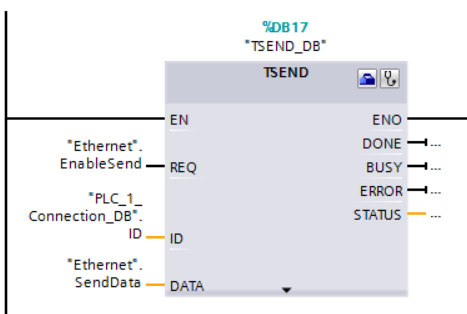
\includegraphics[width=0.5\textwidth]{Figure/TSEND}
	\caption{Blokken TSEND}
	\label{fig:TSEND}
\end{figure}


Med en pålidelig og testet TCP kommunikation var de næste overvejelser angående styringen af disse blokke. Her blev det besluttet, at et client/server forhold ville være bedst. Kontrolmodulet er i den sammenhæng client og skal forespørge data fra serveren, Kommunikationsmodulet.
Da systemet ikke er et beskyttelsessystem, kræver det ikke hurtig reaktion mellem sensor og aktuator. Derfor blev det valgt, at det kun var nødvendigt at opdatere data hvert 2 sekunder. Dette blev realiseret med to separate netværk; et tilknyttet FC'en med TSEND og et tilknyttet FC'en med TRCV. På figur \ref{fig:ValgAfEnhedSend} ses netværket tilknyttet TSEND.

\begin{figure}[H] % (alternativt [H])
	\centering
	\includegraphics[width=1\textwidth]{Figure/valgAfEnhedSend}
	\caption{Netværket der styrer hvilken enhed der forespørges data fra}
	\label{fig:ValgAfEnhedSend}
\end{figure}

FC'er er valgt, da tanken var at hukommelsen skulle ligge andetsteds i koden. Det er dog blevet nødvendigt at oprette en global DB for at kunne styre variable i forbindelse med styring af kommunikationen. For yderlige uddybelse, se dokumentationen\footnote{Projektdokumentation, 10.1.1, TCP kommunikation}.


Det er vigtigt at pointere, at systemet skal være nemt at udvide til at understøtte mange Måleenheder i den virkelige verden. Det vil udvide tiden, det tager at eksekvere programmet, men er nemt, da der ikke skal ændres i selve kommunikationen, men kun i de netværk, der styrer kommunikationen, hvor der her skal tilføjes flere forgreninger.

\subsection{Styring af Trinskifter}

Angående styring af Trinskifteren blev det tidligt besluttet at benytte dens analoge 24VDC udgange på Q0.6, Q0.7 og Q1.0 til styringen af relæerne på Trinskifter. Disse udgange bliver dog styret med et logisk højt (24VDC) eller lavt(0V) signal. Der henvises til Trinskifter for mere om relækredsløbet, se afsnit \ref{sec:relae}.
Samtidig er projektet proof of concept, så det er kun spændingsmålinger fra én forbruger, der vil blive reguleret med hensyn til. Dette simplificerer den FB, der udvikles til denne styring væsentligt, da der kun er et input. På \ref{fig:GraphTrinskifterPLC} ses et diagram over sekvenserne og flowet imellem dem for FB'en Trinskifter.

\begin{figure}[H] % (alternativt [H])
	\centering
	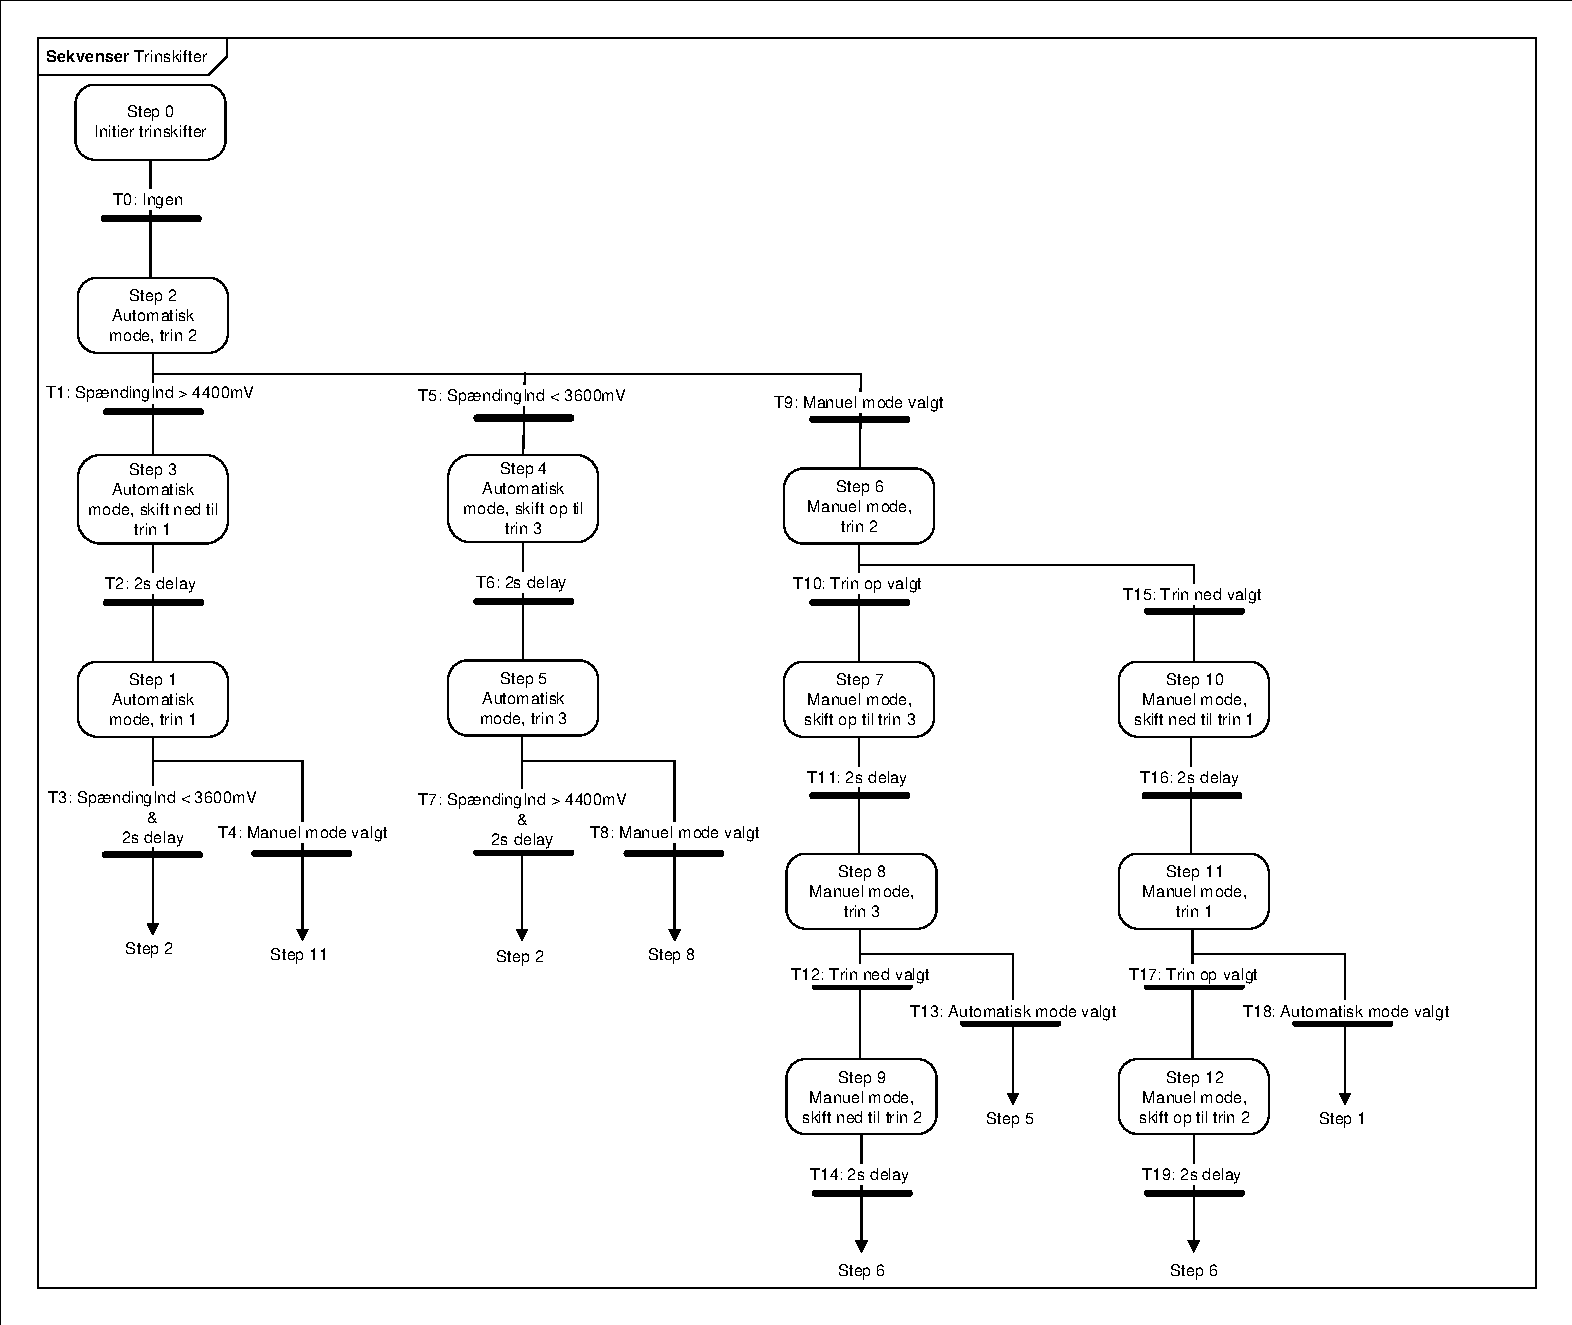
\includegraphics[width=1\textwidth]{Figure/GraphTrinskifterPLC}
	\caption{Diagrammet viser FB'en Trinskifters sekvenser}
	\label{fig:GraphTrinskifterPLC}
\end{figure}

Første tanke i forhold til denne blok var, at den hovedsageligt skulle være automatiseret. Derfor er det besluttet, at koden blev skrevet som sekventiel, hvor en lokal static Step står for at styre, hvilken sekvens der er aktiv. Dette sikrer også imod fejl, da systemet har få muligheder videre fra hvert step. Et sikkert system var også et af de vigtige punkter, hvilket bl.a. er opnået ved at opdele koden i sekvenser af trin og trinskift. Der er 3 trin, som hver især er tilknyttet en af udgangene på PLC'en. For trin 2 er der både mulighed for et trinskift op og ned, mens der for ydertrinene kun kan skiftes ned/op til trin 2. Det er kun, når koden er i et trin, at man kan skifte mellem automatisk og manuel tilstand. I automatisk mode er der dog to undtagelser i trin 1 og trin 3, hvor trinskiftet er lagt sammen med trinet. Disse trinskift burde have været flyttet til deres egen sekvens for at undgå at et trinskift og et tilstandsskift kan forekomme samtidigt.


I første udkast til blokken var der ikke taget højde for at programmet blev eksekveret hurtigere end data blev opdateret, derfor kunne programmet nå at skifte flere trin på den samme måling, hvilket vil skabe et ustabilt system, for når det havde lavet et dobbeltskift, vil det så få en ny måling, der indikerer skift i modsat retning. Denne fejl er fjernet ved at indsætte et delay, når systemet kommer i et nyt trin, da der hentes ny data hvert 2 sekunder, er dette delay sat til 2,5 sekunder.


En vigtig pointe at få med er, at forbrugeren aldrig må miste forsyning. Så et trinskift indebærer et overlap imellem de trin, der skiftes fra og til på 2 sekunder. Herved er der altid forsyning på distributionslinjen. Selve overlappet set fra trintransformeren uddybes i afsnit \ref{sec:ImpTrinskift}.
For mere om styringen af trinskifteren, se dokumentationen.\footnote{Projektdokumentation, 10.1.2, Styring af Trinskifteren.}

% !TEX root = ../../prj4projektrapport.tex
% SKAL STÅ I TOPPEN AF ALLE FILER FOR AT MASTER-filen KOMPILERES 


\section{Brugergrænseflade}

Brugergrænsefladen i dette projekt er designet på en HMI KTP 600. Den kan tilgås gennem en switch af typen CSM 1277. I dette afsnit vil overvejelser omkring HMI'et blive gennemgået, koden og opsætningen er forklaret i dokumentationen.\footnote{Projektdokumentationen, 10.2, Brugergrænseflade}


Systemet der udvikles skulle være operatørvenligt, hvilket har været grundlag for mange beslutninger omkring HMI'et. Det skal være let at gennemskue og der skal kun være de mest nødvendige funktionaliteter, for at give overblik.
Der er derfor fremstillet to skærme; Automatisk mode og Manuel mode. Der er få forskelle på de to, men det tydeliggør for operatøren, hvilken tilstand der er aktiv. Skærmen for Automatisk mode kan ses på figur \ref{fig:HMIAutomatiskModeDesign}. Skærmen for manuel mode kan findes i dokumentationen.\footnote{Projektdokumentationen, 10.2.2, Manuel mode}

\begin{figure}[H] % (alternativt [H])
	\centering
	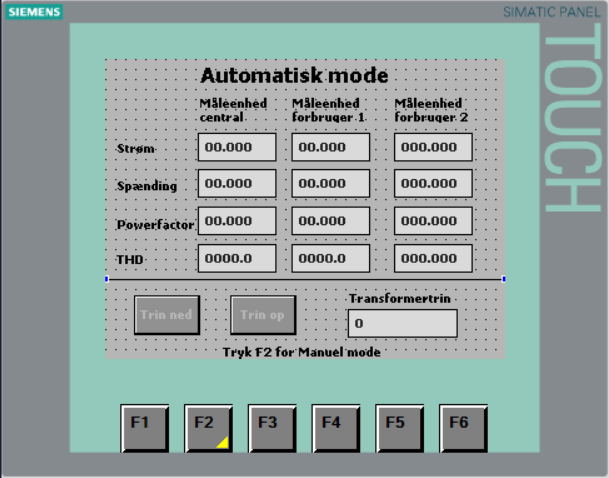
\includegraphics[width=0.7\textwidth]{Figure/HMIAutomatiskModeDesign}
	\caption{HMI i automatisk mode}
	\label{fig:HMIAutomatiskModeDesign}
\end{figure}

På begge skærme vises data for Måleenhederne i kolonner og rækker, for at give overblik. En mangel her er at det ikke er vist hvilken enhed, dataet vises i. For spænding er det i volt, strøm i ampere, power factor er enhedsløs og THD er vises som det samlede indhold af frekvenser i procent af den fundamentale frekvens. THD er forklaret i afsnit \ref{sec:THD}.


Under skillelinjen ses al information omkring Trinskifteren. I automatisk mode er det ikke muligt at skifte trin på knapperne Trin ned og Trin op, derfor er de gråskalerede. I manuel mode er de sort/hvid for at vise at de kan benyttes.


Knappen til tilstandsskift er på hver skærm placeret på F-knapperne med tilhørende forklarende tekst på skærmen, for at tydeliggør funktonaliteten af knapperne.


Systemet er klargjort til at en central og to decentrale Måleenheder, men i det endelige produkt er kun en central og en decentral Måleenhed. Forbruger 2 er derfor ikke aktiv i produktet.
% !TEX root = ../../prj4projektrapport.tex
% SKAL STÅ I TOPPEN AF ALLE FILER FOR AT MASTER-filen KOMPILERES 

\section{Kommunikationsmodul}

I starten af projektet var det tænkt at et separat kommunikationsmodul ikke var nødvendigt, da PSoC'en med et tilhørende Ethernetmodul ENC28J60 burde 

Kommunikationsmodulet består af en Arduino Mega2560 forbundet til et Ethernet Shield R3. Kommunikationsmodulet står for kommunikationen mellem Måleenhederne og Kontrolmodulet, det skal dermed modtage data fra Måleenhederne over UART kommunikation og sende det videre til Kontrolmodulet ved brug af TCP kommunikation. 

Arduinoen opsætter Ethernet Shield'et ved brug af en SPI forbindelse, der oprettes af SPI.h biblioteket, der kaldes som det første i koden. Dernæst er Ethernet.h biblioteket kaldt, for at kunne benytte de meget brugbare funktioner i dette bibliotek. 
% !TEX root =../prj4projektrapport.tex


\section{Delkonklusion}

I kapitel 5 er overvejelser omkring udvikling, design og implementering af Distributionslinje, Belastning og Trinskifter blevet beskrevet. Der er implementeret en simulering af en 60 km lang distributionslinje med modstand- og spolevirkning, der påvirker spændingsfald og power factor i systemet. Ligeledes er der implementeret belastninger, der kan til- og frakobles for at variere spændingsfaldet over disse. Endeligt er der implementeret en trinskifter i form af en trintransformer og et relækredsløb til skift af trin. På baggrund af modultest kan det konkluderes, at disse enheder giver mulighed for at lave det ønskede proof of concept.


\chapter{Integrationstest}
\chapter{Accepttest}
\chapter{Resultat og Diskussion}
\chapter{Metode og proces}
\chapter{Fremtidigt arbejde}
\chapter{Perspektivering}
\chapter{Konklusion}

\printbibliography

\end{document}


